\documentclass[10pt]{amsart}
\usepackage{geometry}                % See geometry.pdf to learn the layout options. There are lots.
\geometry{letterpaper}                   % ... or a4paper or a5paper or ... 
\usepackage{graphicx}
\usepackage{amssymb}
\usepackage{epstopdf}
\usepackage{natbib}
\DeclareGraphicsRule{.tif}{png}{.png}{`convert #1 `dirname #1`/`basename #1 .tif`.png}

\title{Some Solutions to the Planetary Geostrophic Equations}
\author{TWNH}
\date{\today}                                           % Activate to display a given date or no date

\begin{document}
\maketitle

\citet{peterson&callies26} (see also \citealt{peterson&callies23}) consider how bottom-intensified vertical mixing induces a basin-scale circulation in various simple non-flat-bottomed basins.
They write equations for a bottom Ekman layer and couple them to an equation for the geostrophic contour vorticity balance, in the parlance of \citet{waldman&giordani23}, which is a type of barotropic vorticity equation.

\section{Governing Equations}
The flow satisfies the (non-dimensional) planetary-geostrophic equations:
\begin{align}
- f v & = - \frac{\partial p}{\partial x} + \epsilon^2 \frac{\partial}{\partial z} \left( \nu \frac{\partial u}{\partial z} \right), \label{eqn:u_mom} \\
f  u & = - \frac{\partial p}{\partial y} + \epsilon^2 \frac{\partial}{\partial z} \left( \nu \frac{\partial v}{\partial z} \right),  \label{eqn:v_mom} \\
\end{align}
(see Eqs.~(9)--(11) of \citealt{peterson&callies26}, Eq.~(3.26) of \citealt{klinger&haine19}, and Eq.~(2.274) of \citealt{vallis06}).
The boundary conditions are no flow at the bottom and a specified stress at the surface:
\begin{align}
\text{Surface~}z = 0:
\epsilon^2 \nu \partial_z (u, v) & = (\tau^x , \tau^y ), 
 \\
\text{Bottom~}z = -H:
(u, v) & = 0 ,
\end{align}
The flow is non-divergent:
\begin{align}
\nabla \cdot {\mathbf u} & = 0 ,
\label{eqn:non-divergent}
\end{align}
the buoyancy field is hydrostatic:
\begin{align}
\frac{\partial p}{\partial z} & = b ,
\end{align}
and the buoyancy field satisfies the advection-diffusion-relaxation equation
\begin{align}
\mu \rho \left( \frac{\partial b}{\partial t} + {\mathbf u} \cdot \nabla b \right) = \epsilon^2 \frac{\partial }{\partial z} \left( \kappa \frac{\partial b}{\partial z} \right) + \gamma \left( B - b \right).
\label{eqn:b}
\end{align}
(see Eqs.~(11)--(13) of \citealt{peterson&callies26}).
The boundary conditions on buoyancy are:
\begin{align}
\text{Surface~}z = 0:
b &= 0
\label{eqn:sfc_b_bc}
 \\
\text{Bottom~}z = -H:
\frac{\partial b}{\partial z} &= 0 ,
\label{eqn:bot_b_bc}
\end{align}
and the initial condition is $b = z$.
The buoyancy field relaxes to a specified field $B(x, y, z, t)$ with rate $\gamma$.

The diffusivity and viscosity are given by
\begin{align}
\kappa(z) & = \kappa_0 + \exp \left( - \alpha (z + H) \right) , \label{eqn:kappa_def} \\
\nu & = \text{constant}
\end{align}
\citet{peterson&callies26} Eq.~(17).

\section{Vertically-Integrated Flow}
The vertically-integrated flow $(U, V)$ is given by:
\begin{align}
U & \equiv \int_{-H}^{0} u \; dz = - \int_{-H}^0 z \partial_z u \; dz , \nonumber \\
V & \equiv \int_{-H}^{0} v \; dz = - \int_{-H}^0 z \partial_z v \; dz ,
\label{eqn:UV_defs}
\end{align}
exploiting the bottom boundary condition on $(u, v)$.
The equations for $(U, V)$ come from vertically integrating the momentum equations (\ref{eqn:u_mom}), (\ref{eqn:v_mom}):
\begin{align}
- f V & = -  \int_{-H}^{0} \frac{\partial p}{\partial x} \; dz + \epsilon^2   \int_{-H}^{0} \frac{\partial}{\partial z} \left( \nu \frac{\partial u}{\partial z} \right) \; dz \label{eqn:U_mom0} \\
f  U & = -  \int_{-H}^{0} \frac{\partial p}{\partial y} \; dz + \epsilon^2  \int_{-H}^{0} \frac{\partial}{\partial z} \left( \nu \frac{\partial v}{\partial z} \right) \; dz . \label{eqn:V_mom0}
\end{align}
The depth-integrated pressure gradient in the $x$ direction is:
\begin{align}
 \int_{-H}^{0} \frac{\partial p}{\partial x} \; dz & = - \frac{\partial H}{\partial x} p(x,z = -H) +  \frac{\partial }{\partial x} \int_{-H}^0 p \; dz , \\
 & = - p_b \frac{\partial H}{\partial x} + \frac{\partial }{\partial x} \left[ p_b H - \int_{-H}^0 z \frac{\partial p}{\partial z}  \right], \\
  & = H \frac{\partial p_b}{\partial x} - \frac{\partial }{\partial x} \int_{-H}^0 z b \; dz ,
 \end{align}
 using the Liebniz integration formula\footnote{The Liebniz integration formula reads:
 \begin{align}
 \partial_x \left( \int_{a(x)}^{b(x)} f(x,y) \; dy \right) = \partial_x b f(x,b(x)) - \partial_x a f(x,a(x)) +  \int_{a(x)}^{b(x)} \partial_x f(x, y) \; dy . \nonumber
 \end{align}
 }, where $p_b = p(x,-H(x))$ is the bottom pressure, and integration by parts\footnote{
 Integration by parts gives:
 \begin{align}
\int_{-H}^0 z \frac{\partial p}{\partial z} \; dz & = \left[ z p \right]_{-H}^0 -   \int_{-H}^0 p \; dz , \nonumber \\ 
& = p_b H -  \int_{-H}^0 p \; dz . \nonumber
 \end{align}
 }.
 The viscous term in the $x$ direction is:
 \begin{align}
  \int_{-H}^{0} \frac{\partial}{\partial z} \left( \nu \frac{\partial u}{\partial z} \right) \; dz & = \left[  \nu \frac{\partial u}{\partial z}  \right]_{-H}^{0}  = \frac{\tau^x}{ \epsilon^2}  - \left. \nu \frac{\partial u}{\partial z} \right|_{z = -H} ,
 \end{align}
which uses the boundary condition (\ref{eqn:sfc_bcs}).
  
 Therefore (\ref{eqn:U_mom0}) and (\ref{eqn:V_mom0}) lead to the (steady, linear) barotropic momentum equations:
 \begin{align}
- f V & =  - H \frac{\partial p_b}{\partial x} - \frac{\partial \chi}{\partial x}  - \tau^x_b + \tau^x , \label{eqn:U_mom} \\
f  U & = - H \frac{\partial p_b}{\partial y} - \frac{\partial \chi }{\partial y}  - \tau^y_b + \tau^y \label{eqn:V_mom} ,
\end{align}
where
\begin{align}
\chi & = - \int_{-H}^0 z b \; dz
\label{eqn:baroclinic_PE}
\end{align}
is the baroclinic potential energy, and $\epsilon^2  \nu \left. \partial_z (u,v) \right|_{z = -H}  \equiv (\tau^x_b, \tau^y_b) = \tau_b$ is the bottom stress on the fluid (see \citealt{waldman&giordani23} Eq.~(9)).

An alternate form of these equations is
 \begin{align}
- f V & =  - H \frac{\partial p_s}{\partial x} - \int_{-H}^0 \frac{\partial  \lambda(z)}{\partial x} \; dz - \tau^x_b + \tau^x , \label{eqn:U_mom_alt} \\
f  U & = - H \frac{\partial p_s}{\partial y} -  \int_{-H}^0 \frac{\partial \lambda(z) }{\partial y}  \; dz - \tau^y_b + \tau^y \label{eqn:V_mom_alt} ,
\end{align}
\begin{align}
\lambda (z) & = \int_{z}^0 b \; dz
\label{eqn:buoyancy_int}
\end{align}
is the vertically-integrated buoyancy and $p_s = p_b - \int_{-H}^0 \lambda(z) \; dz$ is the surface pressure.


\section{Barotropic Vorticity Equation, Barotropic Divergence Equation, and Geostrophic Contour Vorticity Balance}
\citet{waldman&giordani23} show how to derive the barotropic vorticity equation and the geostrophic vorticity balance.

\subsection{Barotropic vorticity equation}
\label{sect:BVE}
Take the curl of the barotropic momentum equations: $\partial_x$(\ref{eqn:V_mom})-$\partial_y$(\ref{eqn:U_mom}) to give:\footnote{
Recall that 
\begin{align}
{\hat{\mathbf z}} \cdot \left( \nabla \times {\mathbf U} \right) & = \partial_x V - \partial_y U .
\end{align}
}
 \begin{align}
\partial_x \left\{ f  U \right\} - \partial_y \left\{ - f V \right\} & =  
\partial_x \left\{ - H \frac{\partial p_b}{\partial y} - \frac{\partial \chi }{\partial y}  - \tau^y_b + \tau^y \right\} -
\partial_y \left\{ - H \frac{\partial p_b}{\partial x} - \frac{\partial \chi}{\partial x}  - \tau^x_b + \tau^x \right\} \nonumber \\
\implies
f \left( \partial_x   U + \partial_y V \right) + \beta V & =  J(p_b, H) + \hat{\mathbf{z}} \cdot \left( \nabla \times \left( \tau - \tau_b \right) \right) .
\label{eqn:BVE}
\end{align}
This is the balance of terms in the steady, linear barotropic vorticity equation (see \citealt{waldman&giordani23} Eq.~(10)).
In this case, the horizontal divergence of the vertically-integrated flow vanishes.
This constraint comes from (\ref{eqn:non-divergent}), which implies that\footnote{
Note that 
\begin{align}
\partial_x U = \partial_x \int_{H(x)}^0 u(x, z) \; dz = \partial_x H\, u(x,-H(x)) + \int_{-H(x)}^0 \partial_x u \; dz , \nonumber
\end{align}
and 
\begin{align}
 \int_{H(x)}^0 \partial_z w(x, z) \; dz = w(x,0) - w(x, -H(x))  .\nonumber
\end{align}
The top boundary condition on the velocity is $w(x,0)=0$ and the bottom boundary condition is $\mathbf{u} \cdot \nabla H = 0$, implying that
\begin{align}
w(x,-H(x)) = -\left[ u(x,-H(x)) \partial_x H + v(x,-H(x)) \partial_y H \right] \nonumber ,
\end{align}
and therefore the vertically-integrated flow has zero horizontal divergence, which is (\ref{eqn:divUiszero}).
}
\begin{align}
\int_{-H}^0 \partial_x u + \partial_y v + \partial_z w \; dz &= 0 , \nonumber \\
\implies \partial_x U + \partial_y V & = 0 .
\label{eqn:divUiszero}
\end{align}
Thus, for steady solutions we require that
 \begin{align}
 J(p_b, H) + \hat{\mathbf{z}} \cdot \left( \nabla \times \left( \tau - \tau_b \right) \right) -  \beta V & = 0
 \label{eqn:BVE_constraint}
\end{align}
(see \citealt{nost&isachsen03} Eq.~(13))

\subsection{Barotropic divergence equation}
\label{sect:BDE}
Take the horizontal divergence of the barotropic momentum equations: $\partial_x$(\ref{eqn:V_mom})-$\partial_y$(\ref{eqn:U_mom}) to give:
 \begin{align}
\partial_x \left\{ - f V \right\}  + \partial_y \left\{ f  U \right\}& =  
\partial_x \left\{ - H \frac{\partial p_b}{\partial x} - \frac{\partial \chi}{\partial x}  - \tau^x_b + \tau^x \right\} +
\partial_y \left\{ - H \frac{\partial p_b}{\partial y} - \frac{\partial \chi }{\partial y}  - \tau^y_b + \tau^y \right\} \nonumber \\
\implies
f \left( \partial_x V - \partial_y U  \right) - \beta U & =  \nabla p_b \cdot \nabla H + H \nabla^2 p_b + \nabla^2 \chi - \nabla \cdot  \left( \tau - \tau_b \right) .
\end{align}
This is the balance of terms in the steady, linear barotropic divergence equation, which also must be satisfied.


\subsection{Geostrophic Contour Vorticity Balance}
Divide the barotropic momentum equations (\ref{eqn:U_mom})--(\ref{eqn:V_mom}) by water depth $H$:
 \begin{align}
- \frac{f V}{H} & =  - \frac{\partial p_b}{\partial x} - \frac{1}{H} \frac{\partial \chi}{\partial x} + \frac{\tau^x - \tau^x_b}{H}   \\
\frac{f  U}{H} & = - \frac{\partial p_b}{\partial y} - \frac{1}{H} \frac{\partial \chi }{\partial y} + \frac{\tau^y - \tau^y_b}{H} ,
\end{align}
and take the curl
 \begin{align}
\frac{\partial}{\partial y} \left\{- \frac{f V}{H} \right\}  - \frac{\partial}{\partial x} \left\{\frac{f  U}{H} \right\} & = 
\frac{\partial}{\partial y} \left\{ - \frac{\partial p_b}{\partial x} - \frac{1}{H} \frac{\partial \chi}{\partial x}  + \frac{\tau^x - \tau^x_b}{H} \right\} \nonumber. \\
& -  \frac{\partial}{\partial x} \left\{ - \frac{\partial p_b}{\partial y} - \frac{1}{H} \frac{\partial \chi }{\partial y}  + \frac{\tau^y - \tau^y_b}{H} \right\}, \\
\implies
\frac{\partial}{\partial y} \left\{- \frac{f }{H} \frac{\partial \Psi}{\partial x} \right\}  + \frac{\partial}{\partial x} \left\{\frac{f }{H} \frac{\partial \Psi}{\partial y} \right\} & = 
- \frac{\partial}{\partial y} \left\{ \frac{1}{H} \frac{\partial \chi}{\partial x} \right\} + \frac{\partial}{\partial x} \left\{ \frac{1}{H} \frac{\partial \chi }{\partial y}  \right\}  - {\hat{\mathbf z}} \cdot \left( \nabla \times \frac{{\mathbf \tau - \tau_b}}{H} \right), \nonumber \\
\implies
- \frac{\partial}{\partial y} \left(\frac{f }{H} \right) \, \frac{\partial \Psi}{\partial x}  + \frac{\partial}{\partial x} \, \left( \frac{f }{H}  \right) \frac{\partial \Psi}{\partial y} & = 
- \frac{\partial}{\partial y} \left( \frac{1}{H} \right) \, \frac{\partial \chi}{\partial x} + \frac{\partial}{\partial x} \, \left( \frac{1}{H} \right) \frac{\partial \chi }{\partial y}   - {\hat{\mathbf z}} \cdot \left( \nabla \times \frac{{\mathbf \tau - \tau_b}}{H} \right), \label{eqn:GCVB0} \\
\implies
J\left( \frac{f}{H} , \Psi \right)  & =  J \left( \frac{1}{H}, \chi \right)
- {\hat{\mathbf z}} \cdot \left( \nabla \times \frac{{\mathbf \tau - \tau_b}}{H} \right) ,
\label{eqn:GCVB}
\end{align}
for streamfunction of the depth-integrated horizontal flow $\Psi$ where
\begin{align}
V & = \phantom{-} \frac{\partial \Psi}{\partial x}, \nonumber \\
U & = - \frac{\partial \Psi}{\partial y} ,
\label{eqn:streamfunction_def}
\end{align}
and Jacobian $J(A,B) = \partial_x A \, \partial_y B - \partial_y A \, \partial_x B$.
Notice how this recipe (vertically integrate, divide by $H$, then take the curl) eliminates the bottom pressure.
The final result (\ref{eqn:GCVB}) is the same as Eq.~(20) of \citet{peterson&callies26}.
It is called (a simplified form of) the \textbf{geostrophic contour vorticity balance} (GCVB) by \citet{waldman&giordani23}, although \citet{peterson&callies26} call it the ``barotropic vorticity equation''.
It is not the same equation as used by \citet{nost&isachsen03} (which \citet{waldman&giordani23} call the ``transport divergence vorticity balance'').

Notice how the GCVB (\ref{eqn:GCVB}) is an equation for the streamfunction of the depth-integrated flow $\Psi$ given the buoyancy field (and hence the JEBAR term) and the surface and bottom stresses.
The GCVB shows how depth-integrated flow $\Psi$ across $f/H$ contours is driven by (i) the joint effect of baroclinicity and relief (JEBAR), (ii) curl of wind stress divided by $H$, (iii) curl of the bottom stress divided by $H$.

\section{Solution to Frictional Geostrophic Equations in Steady State}
\label{sect:FGE_soln}
Start from (\ref{eqn:u_mom})--(\ref{eqn:v_mom}) and write the pressure as
\begin{align}
p(x,y,z) & = p_s(x,y) + \int_{z}^{0} b(x,y,z') \; dz' , \label{eqn:hydrostatic_p} \\
\implies \partial_x p(x,y,z) & = \partial_x p_s (x, y) + \int_{z}^{0} \partial_x b(x,y,z') \; dz'  \label{eqn:hydrostatic_p_pgf} \\
\implies p_b(x, y) & \equiv p(x, y, z=-H(x,y)) = p_s(x,y) + \int_{-H(x,y)}^{0} b(x,y,z') \; dz' , \label{eqn:pb} 
\end{align}
where $p_s(x,y)$ is the surface pressure (and assuming that $p_s \ll p(-H)$).
Solve these frictional geostrophic equations using a Green's function, defined so that $\mathfrak{u} = u + i v$, thus
\begin{align}
\epsilon^2 \frac{\partial}{\partial z} \left( \nu  \frac{\partial \mathfrak{u}}{\partial z} \right)  - i f  \mathfrak{u} & = \mathfrak{f} ,  \\
\text{Surface~}z = 0:
\epsilon^2 \nu \partial_z \mathfrak{u} & = \tau^x + i \tau^y , \label{eqn:sfc_bcs}
 \\
\text{Bottom~}z = -H:
\mathfrak{u} & = 0 ,
\end{align}
where $\mathfrak{f} = \frac{\partial p}{\partial x} +  i \frac{\partial p}{\partial y}$ is the pressure gradient from (\ref{eqn:hydrostatic_p_pgf}).

The corresponding Green's function satisfies:
\begin{align}
\epsilon^2 \frac{\partial}{\partial z} \left( \nu  \frac{\partial G_\mathfrak{u}}{\partial z} \right)  - i f  G_\mathfrak{u} & = \delta(z - \xi) ,  \\
\text{Surface~}z = 0:
\epsilon^2 \nu \partial_z G_\mathfrak{u} & = 0 ,
 \\
\text{Bottom~}z = -H:
G_\mathfrak{u} & = 0 .
\end{align}
We find that the solution for constant viscosity $\nu = \nu_0$ is:  
\begin{align}
 G_{ \mathfrak{u}}(z;\xi) & = 
\frac{ i^{3/2} \mathrm{e}^{- \sqrt{i} \varphi (z + \xi)} }{2  \nu_0 \epsilon^2 \varphi  \left(1 + \mathrm{e}^{2 \sqrt{i} \varphi H \left(x \right)} \right)}
\begin{cases} 
\displaystyle - \mathrm{e}^{2 \sqrt{i} \varphi \xi} + \mathrm{e}^{2 \sqrt{i} \varphi \left( z + H(x)\right)} + \mathrm{e}^{2 \sqrt{i} \varphi \left( z + \xi + H(x)\right)} - 1
 & \text{for}\: z \leq \xi , \\
\displaystyle - \mathrm{e}^{2 \sqrt{i} \varphi z} + \mathrm{e}^{2 \sqrt{i} \varphi \left( \xi + H(x)\right)} + \mathrm{e}^{2 \sqrt{i} \varphi \left( z + \xi + H(x)\right)} - 1
 & \text{for}\: z \geq \xi ,
\end{cases} , \label{eqn:FG_Gsfn} .
\end{align}
This expression implies the following results, which are used later:
\begin{align}
  G_{ \mathfrak{u}}(z;0) & = 
\frac{ i^{3/2} \mathrm{e}^{- \sqrt{i} \varphi z } }{ \nu_0 \epsilon^2 \varphi  \left(1 + \mathrm{e}^{2 \sqrt{i} \varphi H \left(x \right)} \right))}
\left[ \mathrm{e}^{2 \sqrt{i} \varphi ( z  + H{\left(x \right))}} - 1 \right] , \label{eqn:Guv0} \\
 \int_{-H(x)}^0 G_{ \mathfrak{u}}(z;\xi) \; d \xi & = 
 \frac{i  \left(  1 +  \mathrm{e}^{2 \sqrt{i} \phi  H(x)} -  \mathrm{e}^{\sqrt{i} \phi \left(  z + H(x) \right)} -  \mathrm{e}^{\sqrt{i} \phi \left( H(x) - z \right)} \right)  }{\nu_0 \epsilon^{2}  \phi^{2} \left( 1 + \mathrm{e}^{2 \sqrt{i} \phi H(x)} \right)}
\label{eqn:Guv_int_wrt_xi} \\
 \partial_z \left. G_{ \mathfrak{u}}(z;\xi) \right|_{z = -H(x)} & = 
\frac{- \mathrm{e}^{-\sqrt{i} \varphi (\xi - H(x))  } }{ \nu_0 \epsilon^2 \left(1 + \mathrm{e}^{2 \sqrt{i} \varphi H \left(x \right)} \right)}
\left( 1 + \mathrm{e}^{2 \sqrt{i} \varphi \xi}\right) , \label{eqn:FG_Gsfn_bottom_deriv} \\
 \partial_z \left. G_{ \mathfrak{u}}(z;0) \right|_{z = -H(x)} & = 
\frac{- 2 \mathrm{e}^{\sqrt{i} \varphi H(x)  } }{ \nu_0 \epsilon^2 \left(1 + \mathrm{e}^{2 \sqrt{i} \varphi H \left(x \right)} \right)}
% 15Dec25: CHECK DENOMINATOR. IT USED TO READ sqrt{-i}, WHICH LOOKS WRONG.
 , \label{eqn:FG_Gsfn_bottom_deriv_top}
\end{align}
where $\varphi = \sqrt{\left( f / \nu_0 \right) } / \epsilon$ (see \texttt{Example\_barotropic\_GeostrophicFlow\_v0.2.ipynb} and \texttt{ExampleSolution\_v0.5.ipynb} \#1.1, 1.2, and note that this parameter contains $f$ so is a function of space in principle).
And then 
\begin{align}
\mathfrak{u} (z;x) & = \int_{-H(x)}^{0} G_{ \mathfrak{u}} (z; \xi) \left[ \partial_x p( x, \xi) + i \partial_y p( x, \xi) \right] \; d \xi 
 -   G_{\mathfrak{u}} (z; 0)  \left( \tau^x + i \tau^y \right)  .
 \label{eqn:final_uv}
\end{align}
The baroclinic pressure (due to $b$) adds to the barotropic pressure (due to $p_s(x,y)$) in the integrand of this expression. 
Otherwise, everything else is known (remember that $x$ in these expressions stands for $(x,y)$ in general).
Work on the expression (\ref{eqn:final_uv}) for $\mathfrak{u}$ using (\ref{eqn:hydrostatic_p_pgf}) some more, to avoid the multiple vertical integrals:
\begin{align}
\mathfrak{u} (z;x) & = \int_{-H(x)}^{0} G_{ \mathfrak{u}} (z; \xi) \left[ \left(\partial_x  + i \partial_y \right) \left( p_s (x) + \int_{\xi}^{0} b(x,z') \; dz' \right) \right] \; d \xi  -   G_{\mathfrak{u}} (z; 0)  \left( \tau^x + i \tau^y \right)  , \nonumber \\
& = \left(\partial_x  + i \partial_y \right) p_s (x) \int_{-H(x)}^{0} G_{ \mathfrak{u}} (z; \xi) \; d \xi \nonumber \\
&+ \int_{-H(x)}^{0} G_{ \mathfrak{u}} (z; \xi) \left[ \left(\partial_x  + i \partial_y \right)  \int_{\xi}^{0} b(x,z') \; dz' \right] \; d \xi  \nonumber \\
& -   G_{\mathfrak{u}} (z; 0)  \left( \tau^x + i \tau^y \right)  .
\label{eqn:expanded_form_of_u}
\end{align}
The final term is given by (\ref{eqn:Guv0}) and the integral on the second line is given by (\ref{eqn:Guv_int_wrt_xi}).
The integral on the third line is dealt with in section \ref{sect:linear_B_profile} for a specific relaxation buoyancy field.

Also, the bottom current gradient is given by
\begin{align}
-\partial_z \left. \mathfrak{u} (z;x) \right|_{z = -H(x)} & =  \int_{-H(x)}^{0} 
 \frac{ \mathrm{e}^{-\sqrt{i} \varphi (\xi - H(x))  } }{ \nu_0 \epsilon^2 \left(1 + \mathrm{e}^{2 \sqrt{i} \varphi H \left(x \right)} \right)}
\left( 1 + \mathrm{e}^{2 \sqrt{i} \varphi \xi}\right) 
 \left[ \partial_x p( x, \xi) + i \partial_y p( x, \xi) \right] \; d \xi \nonumber \\
& - \frac{ 2 \mathrm{e}^{\sqrt{i} \varphi H(x)  } }{ \nu_0 \epsilon^2 \left(1 + \mathrm{e}^{2 \sqrt{i} \varphi H \left(x \right)} \right)}
\left( \tau^x + i \tau^y \right) ,
\end{align}
using (\ref{eqn:FG_Gsfn_bottom_deriv}) and (\ref{eqn:FG_Gsfn_bottom_deriv_top}), and therefore the bottom stress $\tau_b$ on the fluid is
\begin{align}
\tau_b = - \nu_0 \epsilon^2 \partial_z \left. \mathfrak{u} (z;x) \right|_{z = -H(x)} & = \int_{-H(x)}^{0} 
\frac{ \mathrm{e}^{-\sqrt{i} \varphi (\xi - H(x))  } }{ 1 + \mathrm{e}^{2 \sqrt{i} \varphi H \left(x \right)} }
\left( 1 + \mathrm{e}^{2 \sqrt{i} \varphi \xi}\right) 
 \left[ \partial_x p( x, \xi) + i \partial_y p( x, \xi) \right] \; d \xi \nonumber \\
&-\frac{ 2 \mathrm{e}^{\sqrt{i} \varphi H(x)  } }{ 1 + \mathrm{e}^{2 \sqrt{i} \varphi H \left(x \right)} }
 \left( \tau^x + i \tau^y \right) .
 \label{eqn:bottom_stress_expression}
 \end{align}
Notice how the derivatives of the surface pressure part of $p$ end up multiplying expressions that are functions of $x$.

Work on the bottom stress expression some more by substituting for the pressure gradient from (\ref{eqn:hydrostatic_p_pgf}):
\begin{align}
\tau_b &=  \int_{-H(x)}^{0} 
\frac{ \mathrm{e}^{-\sqrt{i} \varphi (\xi - H(x))  } }{ 1 + \mathrm{e}^{2 \sqrt{i} \varphi H \left(x \right)} }
\left( 1 + \mathrm{e}^{2 \sqrt{i} \varphi \xi}\right) 
 \left[ \left(\partial_x  + i \partial_y\right) \left( p_s(x) + \int_{\xi}^{0} b(x,z') \; dz'  \right) \right] \; d \xi \nonumber \\
&-\frac{ 2 \mathrm{e}^{\sqrt{i} \varphi H(x)  } }{ 1 + \mathrm{e}^{2 \sqrt{i} \varphi H \left(x \right)} }
 \left( \tau^x + i \tau^y \right) .
 \label{eqn:complex_vertical_int_momentum}
 \end{align}
 The integral of the surface pressure term can be computed:
\begin{align}
\int_{-H(x)}^{0} 
\frac{ \mathrm{e}^{-\sqrt{i} \varphi (\xi - H(x))  } }{ 1 + \mathrm{e}^{2 \sqrt{i} \varphi H \left(x \right)} }
\left( 1 + \mathrm{e}^{2 \sqrt{i} \varphi \xi}\right) 
 \left[ \left(\partial_x  + i \partial_y\right)  p_s(x)  \right] \; d \xi & =
 \left[ \left(\partial_x  + i \partial_y\right)  p_s(x)  \right]  \int_{-H(x)}^{0} 
\frac{ \mathrm{e}^{-\sqrt{i} \varphi (\xi - H(x))  } }{ 1 + \mathrm{e}^{2 \sqrt{i} \varphi H \left(x \right)} }
\left( 1 + \mathrm{e}^{2 \sqrt{i} \varphi \xi}\right) 
 \; d \xi \nonumber \\
 & = \frac{1}{\sqrt{i} \varphi} \tanh \left( \sqrt{i} \varphi H(x) \right)   \left[ \left(\partial_x  + i \partial_y\right)  p_s(x)  \right] .
 \end{align}
 Thus,
 \begin{align}
\tau_b &= 
\frac{1}{\sqrt{i} \varphi} \tanh \left( \sqrt{i} \varphi H(x) \right)   \left[ \left(\partial_x  + i \partial_y\right)  p_s(x)  \right] +
 \int_{-H(x)}^{0} 
\frac{ \mathrm{e}^{-\sqrt{i} \varphi (\xi - H(x))  } }{ 1 + \mathrm{e}^{2 \sqrt{i} \varphi H \left(x \right)} }
\left( 1 + \mathrm{e}^{2 \sqrt{i} \varphi \xi}\right) 
 \left[ \left(\partial_x  + i \partial_y\right)  \int_{\xi}^{0} b(x,z') \; dz'   \right] \; d \xi \nonumber \\
&-\frac{ 2 \mathrm{e}^{\sqrt{i} \varphi H(x)  } }{ 1 + \mathrm{e}^{2 \sqrt{i} \varphi H \left(x \right)} }
 \left( \tau^x + i \tau^y \right) , \nonumber \\
\tau_b &=  S(x) \left[ \left(\partial_x  + i \partial_y\right)  p_s(x)  \right] + T(x) ,
 \end{align}
 where
 \begin{align}
S(x) &= 
\frac{1}{\sqrt{i} \varphi} \tanh \left( \sqrt{i} \varphi H(x) \right)  , \nonumber \\
T(x) & = \int_{-H(x)}^{0} 
\frac{ \mathrm{e}^{-\sqrt{i} \varphi (\xi - H(x))  } }{ 1 + \mathrm{e}^{2 \sqrt{i} \varphi H \left(x \right)} }
\left( 1 + \mathrm{e}^{2 \sqrt{i} \varphi \xi}\right) 
 \left[ \left(\partial_x  + i \partial_y\right)  \int_{\xi}^{0} b(x,z') \; dz'   \right] \; d \xi 
-\frac{ 2 \mathrm{e}^{\sqrt{i} \varphi H(x)  } }{ 1 + \mathrm{e}^{2 \sqrt{i} \varphi H \left(x \right)} }
 \left( \tau^x + i \tau^y \right) . 
 \label{eqn:T_fn}
 \end{align} 
 
For an unstratified, flat-bottomed fluid ($\chi = 0, \nabla p_b = \nabla p_s, H = H_0$), specifying the surface pressure gradient $\nabla p_s$ closes the problem. 
We compute the surface stress from (\ref{eqn:complex_vertical_int_momentum}) by substituting (\ref{eqn:bottom_stress_expression}).
Then $u(z), v(z), U, V$ and the force balance can all be computed. 
See Figure \ref{fig:example_soln} for an example calculation..
Alternatively, the surface stress can be specified, and the pressure gradient can be computed (see \texttt{Example\_barotropic\_GeostrophicFlow\_v0.3.ipynb}).
In practice, it seems that the bottom stress always vanishes. Why??  Is this correct??


\begin{figure}
\centering
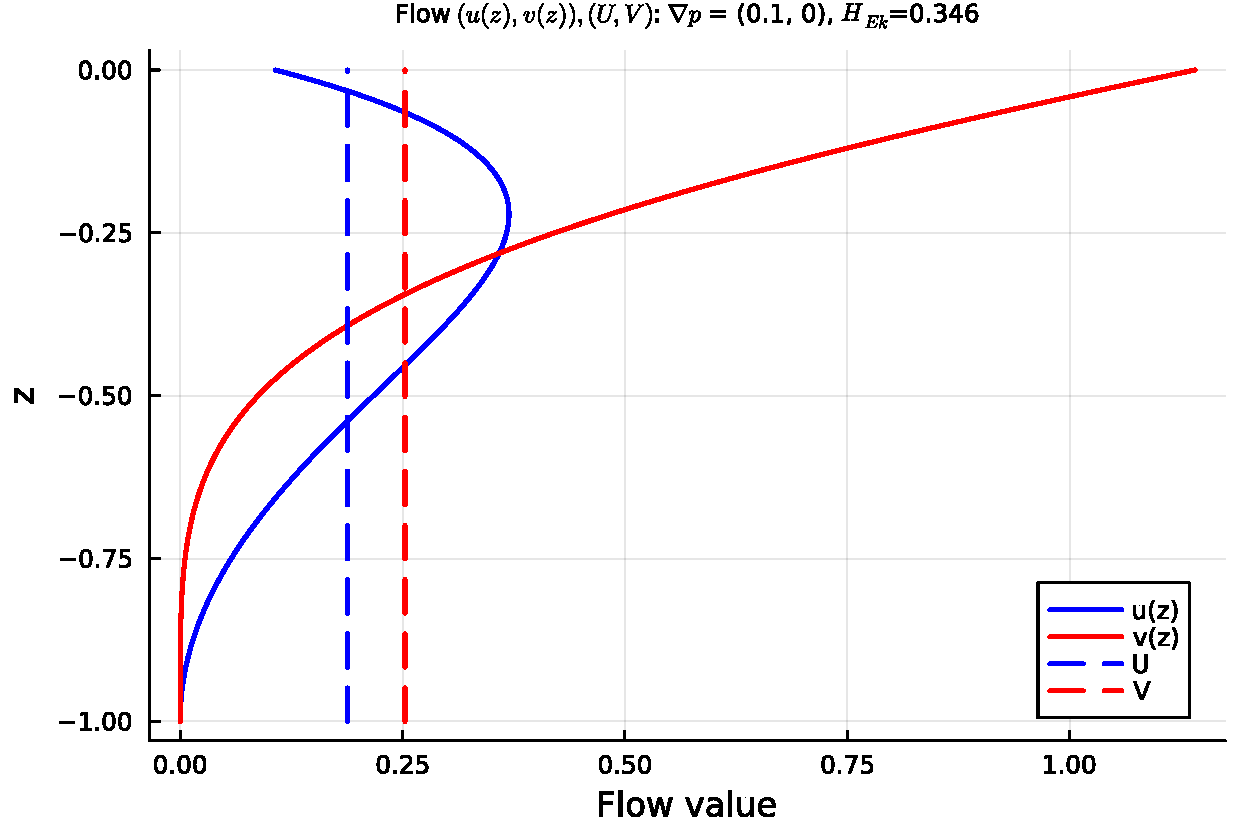
\includegraphics[width=9cm]{Example_barotropic_GeostrophicFlow_v0.2.ipynb_VerticalProfiles.pdf}
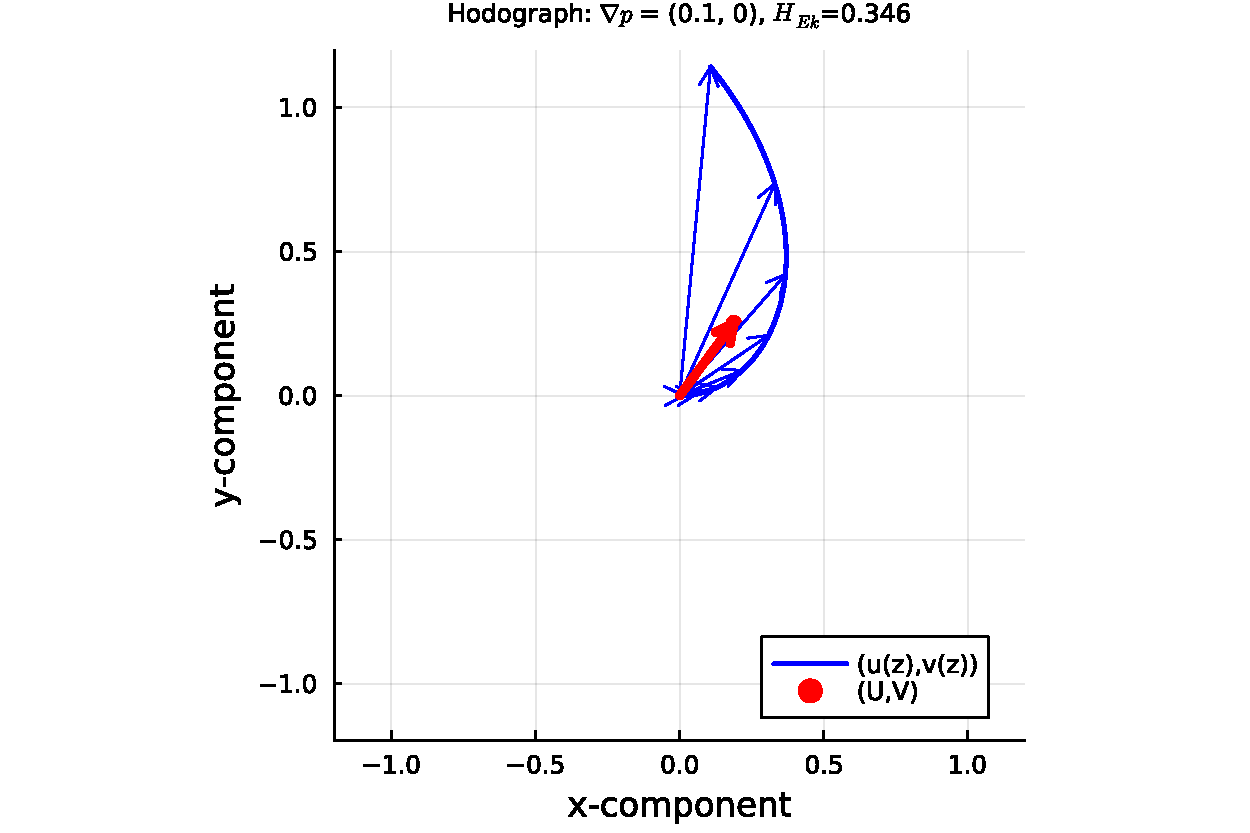
\includegraphics[width=12cm]{Example_barotropic_GeostrophicFlow_v0.2.ipynb_Hodograph.pdf}
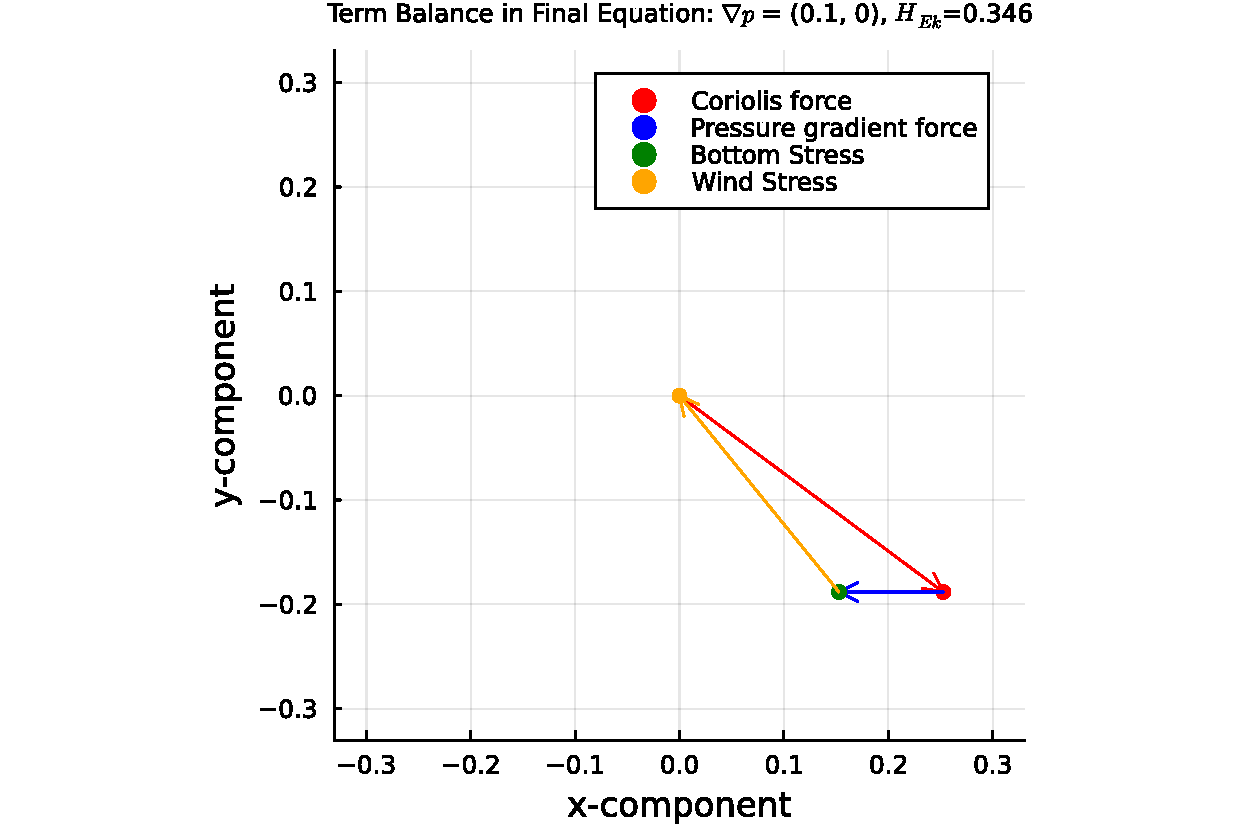
\includegraphics[width=12cm]{Example_barotropic_GeostrophicFlow_v0.2.ipynb_TermBalance.pdf}
\caption{\label{fig:example_soln} Example solution to the barotropic frictional geostrophic flow problem from \texttt{Example\_barotropic\_GeostrophicFlow\_v0.2.ipynb}. See also Figure 2.12 from \citet{vallis06}.}
\end{figure}


\section{Frictional Geostrophic Equations Closure with the Barotropic Momentum Equation}
\label{sect:FGE_closure}

The problem is closed using the barotropic momentum equation, as follows (\citealt{salmon98}, p.~170).
This determines the unknown surface pressure field given the surface stress (and vice versa).
In particular, work from (\ref{eqn:U_mom})--(\ref{eqn:V_mom}),
\begin{align}
\mathfrak{U} (z;x) & \equiv U + i V = \int_{-H(x)}^{0} \mathfrak{u} (z;x) \; dz , \label{eqn:depth_integrated_flow_def} \\
& = \int_{-H(x)}^0 \left\{ \int_{-H(x)}^{0} G_{ \mathfrak{u}} (z; \xi) \left[ \partial_x p( x, \xi) + i \partial_y p( x, \xi) \right] \; d \xi 
-  G_{\mathfrak{u}} (z; 0)  \left( \tau^x + i \tau^y \right)  \right\} \; dz.
\end{align}
Computing the $z$ integral of the Green's function $G_{\mathfrak{u}} (z; \xi)$\footnote{This presumes (correctly) that the denominator in (\ref{eqn:FG_Gsfn}) does not vanish.} gives 
\begin{align}
\int_{-H(x)}^0 G_{ \mathfrak{u}}(z;\xi) \; dz & = 
\frac{- i \mathrm{e}^{-\sqrt{i} \varphi \xi} 
\left(
\mathrm{e}^{\sqrt{i} \varphi \xi} - 
\mathrm{e}^{\sqrt{i} \varphi H(x)} 
\right) \left(
\mathrm{e}^{\sqrt{i} \varphi  \left( \xi + H(x) \right)} - 1
\right)
} { \nu_0 \epsilon^2 \varphi^2  \left(1 + \mathrm{e}^{2 \sqrt{i} \varphi H(x )} \right)} , \nonumber \\
\implies \int_{-H(x)}^0 G_{ \mathfrak{u}}(z;0) \; dz & = 
\frac{ - i \left( 
\mathrm{e}^{\sqrt{i} \varphi  H(x) }   - 1   
\right)^2
} { \nu_0 \epsilon^2 \varphi^2  \left(1 + \mathrm{e}^{2 \sqrt{i} \varphi H(x )} \right)} .
\end{align}
Therefore,
\begin{align}
\mathfrak{U} (x) & = 
\frac{-i }{{ f  \left(1 + \mathrm{e}^{2 \sqrt{i} \varphi H(x )} \right)} } \times \nonumber \\
&\left\{
 \int_{-H(x)}^{0} 
\mathrm{e}^{-\sqrt{i} \varphi \xi} 
\left(
\mathrm{e}^{\sqrt{i} \varphi \xi} - 
\mathrm{e}^{\sqrt{i} \varphi H(x)} 
\right) \left(
\mathrm{e}^{\sqrt{i} \varphi  \left( \xi + H(x) \right)} - 1
\right)
 \left[ \partial_x p( x, \xi) + i \partial_y p( x, \xi) \right] \; d \xi  \right. \nonumber  \\
& + \left.
\left( 
\mathrm{e}^{\sqrt{i} \varphi  H(x) }   - 1   
\right)^2
\left( \tau^x + i \tau^y \right)   \right\}
\label{eqn:UV_expression}
\end{align}
(see \texttt{PlanetaryGeostrophicTheory\_v0.2.ipynb}).
Substituting for the pressure gradient from (\ref{eqn:hydrostatic_p}) then gives:
\begin{align}
\mathfrak{U} (x) & = 
\frac{-i }{{ f  \left(1 + \mathrm{e}^{2 \sqrt{i} \varphi H(x )} \right)} } \times \nonumber \\
&\left\{
 \int_{-H(x)}^{0} 
\mathrm{e}^{-\sqrt{i} \varphi \xi} 
\left(
\mathrm{e}^{\sqrt{i} \varphi \xi} - 
\mathrm{e}^{\sqrt{i} \varphi H(x)} 
\right) \left(
\mathrm{e}^{\sqrt{i} \varphi  \left( \xi + H(x) \right)} - 1
\right)
 \left[ \left( \partial_x + i \partial_y \right) \left( p_s(x) + \int_{\xi}^{0} b(x,z') \; dz' \right)  \right] \; d \xi  \right. \nonumber  \\
& + \left.
\left( 
\mathrm{e}^{\sqrt{i} \varphi  H(x) }   - 1   
\right)^2
\left( \tau^x + i \tau^y \right)   \right\} .
\end{align}
The integral of the surface pressure term can be computed:
\begin{align}
 \int_{-H(x)}^{0} 
\mathrm{e}^{-\sqrt{i} \varphi \xi} 
\left(
\mathrm{e}^{\sqrt{i} \varphi \xi} - 
\mathrm{e}^{\sqrt{i} \varphi H(x)} 
\right) \left(
\mathrm{e}^{\sqrt{i} \varphi  \left( \xi + H(x) \right)} - 1
\right)
 \left[ \left( \partial_x + i \partial_y \right) p_s(x)  \right] \; d \xi  \nonumber  \\
= 
 \left[ \left( \partial_x + i \partial_y \right) p_s(x)  \right] 
 \left[
 - H(x) \left( \mathrm{e}^{2 \sqrt{i} \varphi H(x)} + 1 \right) + \frac{ \mathrm{e}^{2 \sqrt{i} \varphi H(x)}  -1  }{\sqrt{i} \varphi}
 \right]  \nonumber
\end{align}
(see \texttt{ExampleSolution\_v0.2.ipynb}).
Therefore,
\begin{align}
\mathfrak{U} (x) & = 
\frac{-i }{{ f \left(1 + \mathrm{e}^{2 \sqrt{i} \varphi H(x )} \right)} } \times \nonumber \\
&\Bigg\{
 \left[ \left( \partial_x + i \partial_y \right) p_s(x)  \right] 
 \left[
 - H(x) \left( \mathrm{e}^{2 \sqrt{i} \varphi H(x)} + 1 \right) + \frac{ \mathrm{e}^{2 \sqrt{i} \varphi H(x)}  -1  }{\sqrt{i} \varphi}
 \right] + 
 \nonumber \\
 & 
 \int_{-H(x)}^{0} 
\mathrm{e}^{-\sqrt{i} \varphi \xi} 
\left(
\mathrm{e}^{\sqrt{i} \varphi \xi} - 
\mathrm{e}^{\sqrt{i} \varphi H(x)} 
\right) \left(
\mathrm{e}^{\sqrt{i} \varphi  \left( \xi + H(x) \right)} - 1
\right)
 \left[ \left( \partial_x + i \partial_y \right) \int_{\xi}^{0} b(x,z') \; dz'  \right] \; d \xi   \nonumber  \\
& +
\left( 
\mathrm{e}^{\sqrt{i} \varphi  H(x) }   - 1   
\right)^2
\left( \tau^x + i \tau^y \right)   \Bigg\} \nonumber \\
\implies \mathfrak{U} &= U + iV =
A(x)\,\left( \partial_x + i \partial_y \right) p_s(x)  + B(x) ,
\label{eqn:UV_expression3}
\end{align}
where
\begin{align}
A(x) & = 
\frac{-i }{{ f  \left(1 + \mathrm{e}^{2 \sqrt{i} \varphi H(x )} \right)} } 
\left[  - H(x) \left( \mathrm{e}^{2 \sqrt{i} \varphi H(x)} + 1 \right) + \frac{ \mathrm{e}^{2 \sqrt{i} \varphi H(x)}  -1  }{\sqrt{i} \varphi} \right]
, \nonumber \\
A(x) & = 
\frac{i }{{ f  } } 
\left[  H(x)  + \frac{ 1 - \mathrm{e}^{2 \sqrt{i} \varphi H(x)}  }{\sqrt{i} \varphi  \left(1 + \mathrm{e}^{2 \sqrt{i} \varphi H(x )} \right)} \right]
, \nonumber \\
B(x) & =
\frac{-i }{{ f  \left(1 + \mathrm{e}^{2 \sqrt{i} \varphi H(x )} \right)} } 
\Bigg[ \int_{-H(x)}^{0} 
\mathrm{e}^{-\sqrt{i} \varphi \xi} 
\left(
\mathrm{e}^{\sqrt{i} \varphi \xi} - 
\mathrm{e}^{\sqrt{i} \varphi H(x)} 
\right) \left(
\mathrm{e}^{\sqrt{i} \varphi  \left( \xi + H(x) \right)} - 1
\right)
 \left[ \left( \partial_x + i \partial_y \right) \int_{\xi}^{0} b(x,z') \; dz'  \right] \; d \xi   \nonumber  \\
& +
\left( 
\mathrm{e}^{\sqrt{i} \varphi  H(x) }   - 1   
\right)^2
\left( \tau^x + i \tau^y \right)  , \Bigg]  
\label{eqn:B_fn}
\end{align}
(see \texttt{ExampleSolution\_v0.2.ipynb} to verify these expressions, and notice that this $B(x)$ is not the same as the relaxation buoyancy profile $B(z)$ used in section \ref{sec:b_solution}).
%\footnote{Notice that the integral in the $B(x)$ term can be written as:
%\begin{align}
%&  
%\int_{-H(x)}^{0} 
%\left(
%1 - 
%\mathrm{e}^{\sqrt{i} \varphi \left( \xi - H(x) \right)} 
%\right) \left(
%\mathrm{e}^{\sqrt{i} \varphi  \left( \xi + H(x) \right)} - 1
%\right)
% \left[ \left( \partial_x + i \partial_y \right) \int_{\xi}^{0} b(x,z') \; dz'  \right] \; d \xi  \nonumber  \\
% & = 
% \int_{-H(x)}^{0} 
%\mathrm{e}^{\sqrt{i} \varphi  \left( \xi + H(x) \right)} - 1 - \mathrm{e}^{ 2 \sqrt{i} \varphi  \xi } + \mathrm{e}^{\sqrt{i} \varphi \left( \xi - H(x) \right)} 
% \left[ \left( \partial_x + i \partial_y \right) \int_{\xi}^{0} b(x,z') \; dz'  \right] \; d \xi   \nonumber \\
%  & = 
%\left[
%\mathrm{e}^{\sqrt{i} \varphi  H(x)}  + \mathrm{e}^{- \sqrt{i} \varphi  H(x)} \right]
%\int_{-H(x)}^{0} \mathrm{e}^{\sqrt{i} \varphi  \xi } \left[ \left( \partial_x + i \partial_y \right) \int_{\xi}^{0} b(x,z') \; dz'  \right] \; d \xi    \nonumber \\
%& -   \int_{-H(x)}^{0} \left( \partial_x + i \partial_y \right) \int_{\xi}^{0} b(x,z') \; dz'   \; d \xi    \nonumber \\
% & - \int_{-H(x)}^{0} \mathrm{e}^{ 2 \sqrt{i} \varphi  \xi }  \left[ \left( \partial_x + i \partial_y \right) \int_{\xi}^{0} b(x,z') \; dz'  \right] \; d \xi \nonumber .
%\end{align}
%This might be useful in solving the problem numerically.
%}

This formula expresses the depth-integrated flow in terms of the applied surface stress and the buoyancy field (in $B(x)$) and the surface pressure field.
The $A(x)$ field only depends on the fluid depth $H(x)$.
Note also that the streamfunction for the depth-integrated flow (\ref{eqn:streamfunction_def}) is given by:
\begin{align}
\nabla^2 \Psi & =  - \left( i \partial_x + \partial_y \right) \mathfrak{U} , \nonumber \\
& =  - \left( i \partial_x + \partial_y \right) \left[ A(x)\,\left( \partial_x + i \partial_y \right) p_s(x)  + B(x) \right] .
\label{eqn:streamfunction_pde}
\end{align}

To close the problem, utilize the constraint that the vertically-integrated flow is non-divergent (\ref{eqn:non-divergent}).
This requirement amounts to (from (\ref{eqn:BVE_constraint})):
\begin{align}
\Re \left\{ \left( \partial_x - i \partial_y \right) \mathfrak{U}(x) \right\} & = 0 , \nonumber 
\end{align}
which implies that
\begin{align}
\Re \big\{ 
\left(
\partial_x - i \partial_y
\right)
\left[
A(x)\,\left( \partial_x + i \partial_y \right) p_s(x)  + B(x) 
\right]
\big\} & = 0 \nonumber
\end{align}
from (\ref{eqn:UV_expression3}).
The final equation for the surface pressure is thus
\begin{align}
\Re \big\{ 
\partial_x 
\left[
A(x) \partial_x p_s(x) + i A(x) \partial_y  p_s(x)  
\right]
 -
i \partial_y
\left[
A(x) \partial_x p_s(x) + i A(x) \partial_y  p_s(x) 
\right]
\big\}
 & = - \Re \big\{ \left(
\partial_x - i \partial_y
\right) B(x) \big\}
 \nonumber \\
 \implies
\Re \big\{ 
\partial_x A(x) \partial_x p_s(x) + A(x) \partial_{xx} p_s(x) +
i  \partial_x A(x) \partial_y  p_s(x) 
& - \nonumber \\
i \partial_y A(x) \partial_x p_s(x)
+  \partial_yA(x) \partial_y  p_s(x) + A(x) \partial_{yy}  p_s(x) 
\big\}
 & =-  \Re \big\{ \left(
\partial_x - i \partial_y
\right) B(x) \big\} .
\end{align}
 This equation is a 2nd-order elliptic equation for $p_s(x)$ given the surface stress and the buoyancy field.
In more compact form, this is the real parts of:
\begin{align}
A \left( \partial_{xx} + \partial_{yy} \right) p_s +
\partial_x A \partial_x p_s +  \partial_y A \partial_y  p_s  +
i \left(  \partial_x A \partial_y  p_s - \partial_y A \partial_x p_s \right)
 & =-  \left(
\partial_x - i \partial_y
\right) B
 \end{align}
 To write the weak form, which is used to compute $p_s$ solutions numerically, take the divergence form of the equation, multiply by test function $v(x)$, and integrate over all space:
 \begin{align}
 \int_{x,y} v
\left(
\partial_x - i \partial_y
\right)
\left[
A\,\left( \partial_x + i \partial_y \right) p_s
\right]
 \; dy\; dx 
 & = \int_{x,y} v \left(
- \partial_x + i \partial_y
\right) B
 \; dy\; dx , \nonumber \\
 \implies
  \int_{x,y} 
\left(
\partial_x - i \partial_y
\right) v
\left[
A\,\left( \partial_x + i \partial_y \right) p_s
\right]
 \; dy\; dx 
 & = \int_{x,y} B \left(
- \partial_x + i \partial_y
\right) v
 \; dy\; dx 
\end{align}
assuming that $p_s$ and $v$ vanish on the boundaries.
Similarly, the weak form to find the streamfunction for the depth-integrated flow, $\Psi$, is (from (\ref{eqn:streamfunction_pde})):
 \begin{align}
 \int_{x,y} v
\nabla^2 \Psi \; dy\; dx 
 & = \int_{x,y} v \left(
- \left( i \partial_x + \partial_y \right) \left[ A(x)\,\left( \partial_x + i \partial_y \right) p_s(x)  + B(x) \right] 
\right) \; dy\; dx , \nonumber \\
 \implies 
 \int_{x,y} \nabla \Psi \cdot \nabla v \; dy \; dx
 & = - \int_\Omega C(x) \, (i\partial_x + \partial_y)v \; d y \; dx , \nonumber
\end{align}
where
\begin{align}
C(x) = A(x) (\partial_x + i\partial_y)p_s(x) + B(x) . \nonumber
\end{align}
assuming that $\Psi$ and $v$ vanish on the boundaries.


\section{Solution to Linear Buoyancy Equation in Steady State}
\label{sec:b_solution}

At least for steady state and negligible buoyancy advection, the buoyancy equation (\ref{eqn:b}) reads:
\begin{align}
\epsilon^2 \frac{\partial }{\partial z} \left( \kappa \frac{\partial b}{\partial z} \right) + \gamma \left(  B(z) - b \right) & = 0, \label{eqn:steady_vertical_b} \\
\text{Surface~}z = 0:
b &= 0
 \\
\text{Bottom~}z = -H:
\frac{\partial b}{\partial z} &= 0
\end{align}
for buoyancy profile $B(z)$ (in principle, $B$ could depend on $(x,y)$ too) and relaxation coefficient $\gamma$, and vertical buoyancy gradient at the sea bed is zero. 
The internal buoyancy source allows for steady-state solutions that have non-trivial solutions (the $t\rightarrow \infty$ solution to (\ref{eqn:b})--(\ref{eqn:bot_b_bc}) is vanishing $b$ everywhere; the \citealt{peterson&callies26} solutions are transient, relaxing to zero).
This problem (\ref{eqn:steady_vertical_b}) can be solved exactly using a Green's function, at least for constant diffusivity, and I suspect also for diffusivity given by (\ref{eqn:kappa_def}). 

In detail: Solve the Green's function problem first:
\begin{align}
\frac{\epsilon^2}{\gamma} \frac{\partial }{\partial z} \left( \kappa \frac{\partial G_b}{\partial z} \right) -  G_b & =  -  \delta(z - \xi) , \label{eqn:Gsfn}\\
\text{Surface~}z = 0:
G_b &= 0 ,
\label{eqn:Gsfn_sfcbc} \\
\text{Bottom~}z = -H:
\frac{\partial G_b}{\partial z} &= 0 .
\label{eqn:Gsfn_botbc}
\end{align}
This is a second order linear ordinary differential equation with two boundary conditions, which can be solved exactly.
The solution for constant diffusivity $\kappa = \kappa_0$ is:
\begin{align}
G_b (z; \xi) & = \frac{\mathrm{e}^{\psi \left(z + \xi\right)}}
{2  \kappa_0 \psi \left(\mathrm{e}^{2 \psi H \left(x \right)} + 1\right)}
\begin{cases} 
\displaystyle \left(1 - \mathrm{e}^{- 2 \psi \xi} \right) \left(\mathrm{e}^{2 \psi H{\left(x \right)}} + \mathrm{e}^{- 2 \psi z  }\right) & \text{for}\: z \leq \xi , \\
\displaystyle \left(1 - \mathrm{e}^{- 2 \psi   z} \right) \left(\mathrm{e}^{2 \psi H{\left(x \right)}} + \mathrm{e}^{- 2 \psi \xi}\right) & \text{for}\: z \geq \xi ,
\end{cases}
\end{align}
with $\psi = \sqrt{\gamma/\kappa_0} / \epsilon$.
Therefore, given $G_b(z; \xi)$,
\begin{align}
b(z; x) = - \gamma \int_{-H(x)}^{0} G_b(z; \xi) B(\xi; x) \; d \xi  .
\label{eqn:b_solution}
\end{align}
See \texttt{DiffusionEquationSolution.ipynb} and \texttt{FindBuoyancyField\_and\_GeostrophicFlow\_v0.?.ipynb} and \texttt{ExampleSolution\_v0.5.ipynb}.

In solving the momentum equations, one needs horizontal derivatives of the vertically-integrated buoyancy field to compute the pressure gradient (\ref{eqn:hydrostatic_p_pgf}).
We need this term:
\begin{align}
 \int_{z}^{0} \partial_x b(x,y,z') \; dz' & = - \gamma \int_{z}^{0} \partial_x  \int_{-H(x)}^{0} G_b(z'; \xi) B(\xi; x) \; d \xi\; dz' , \nonumber \\
 & = - \gamma  \partial_x  \int_{-H(x)}^{0} \left[ \int_{z}^{0} G_b(z'; \xi) \; dz' \right] B(\xi; x) \; d \xi. \nonumber
\end{align}
The integral in square brackets can be computed analytically.
One finds that:
\begin{align}
& \int_{z}^{0} G_b(z'; \xi) \; dz'   =  \frac{1}{ 2 \kappa_0  \psi^{2} \epsilon^{2} \left( \mathrm{e}^{2 \psi H\left( x \right)} + 1 \right) }\bigg[ \nonumber \\
& \mathrm{e}^{\psi \left( z  - \xi + 2  H(x)\right)} -
 \mathrm{e}^{\psi \left( z + \xi + 2 H(x)\right)} +
2 \mathrm{e}^{\psi \left( \xi + 2  H(x) \right) } + 
2 \mathrm{e}^{ - \xi \psi} +  
\mathrm{e}^{  \psi \left(  \xi - z \right)} - 
\mathrm{e}^{ - \psi \left( z + \xi \right)} - \nonumber \\
& \mathrm{e}^{ \psi \left( \xi + 2  H(x) -  \mathrm{Max}\left( z, \xi \right)\right)} - 
\mathrm{e}^{ - \psi \left( \xi - 2  H(x) -  \mathrm{Max}\left( z, \xi \right) \right)} -
\mathrm{e}^{ \psi \left( \xi  -  \mathrm{Max}\left( z, \xi \right) \right)} - 
 \mathrm{e}^{ - \psi \left( \xi - \mathrm{Max}\left( z, \xi \right) \right)} 
\bigg] \nonumber 
\end{align}
(see \texttt{ExampleSolution\_v0.5.ipynb}, \#1.1).

\subsection{Example linear $B(z)$ profile}
\label{sect:linear_B_profile}
For a linear $B(z)$ function, $B(z) = \alpha z$, we have (from (\ref{eqn:b_solution})):
\begin{align}
\frac{ b(x,y,z')}{- \alpha \gamma } & = \int_{-H(x)}^{0} G_b(z; \xi) \xi \; d \xi \nonumber \\
 & =  
 \frac{1}{\kappa_0 \psi^{2} \epsilon^{2} }
 \left[
\frac{ \mathrm{e}^{\psi H(x)} \left( \mathrm{e}^{\psi   z }  -  \mathrm{e}^{- \psi z } \right) }{\psi \left(  \mathrm{e}^{2 \psi H(x)} + 1 \right)} - z
\right]
\end{align}
(see \texttt{ExampleSolution\_v0.5.ipynb} \#2.7).
Also,
\begin{align}
 \int_{z}^{0} \partial_x b(x,y,z') \; dz' 
 & = \frac{- \alpha  \gamma}{2 \kappa_0  \psi^{2} \epsilon^{2}} \,  \partial_x  \int_{-H(x)}^{0} 
\frac{ \xi}{  \mathrm{e}^{2 \psi H\left( x \right)} + 1  }\bigg[ \nonumber \\
& \mathrm{e}^{\psi \left( z  - \xi + 2  H(x)\right)} -
 \mathrm{e}^{\psi \left( z + \xi + 2 H(x)\right)} +
2 \mathrm{e}^{\psi \left( \xi + 2  H(x) \right) } + 
2 \mathrm{e}^{ - \xi \psi} +  
\mathrm{e}^{  \psi \left(  \xi - z \right)} - 
\mathrm{e}^{ - \psi \left( z + \xi \right)} - \nonumber \\
& \mathrm{e}^{ \psi \left( \xi + 2  H(x) -  \mathrm{Max}\left( z, \xi \right)\right)} - 
\mathrm{e}^{ - \psi \left( \xi - 2  H(x) -  \mathrm{Max}\left( z, \xi \right) \right)} -
\mathrm{e}^{ \psi \left( \xi  -  \mathrm{Max}\left( z, \xi \right) \right)} - 
 \mathrm{e}^{ - \psi \left( \xi - \mathrm{Max}\left( z, \xi \right) \right)} 
\bigg]
 \; d \xi \nonumber .
 \end{align}
Now, 
\begin{align}
&\int_{-H(x)}^{0} 
\frac{ \xi}{  \mathrm{e}^{2 \psi H\left( x \right)} + 1  }\bigg[ \nonumber \\
& \mathrm{e}^{\psi \left( z  - \xi + 2  H(x)\right)} -
 \mathrm{e}^{\psi \left( z + \xi + 2 H(x)\right)} +
2 \mathrm{e}^{\psi \left( \xi + 2  H(x) \right) } + 
2 \mathrm{e}^{ - \xi \psi} +  
\mathrm{e}^{  \psi \left(  \xi - z \right)} - 
\mathrm{e}^{ - \psi \left( z + \xi \right)} - \nonumber \\
& \mathrm{e}^{ \psi \left( \xi + 2  H(x) -  \mathrm{Max}\left( z, \xi \right)\right)} - 
\mathrm{e}^{ - \psi \left( \xi - 2  H(x) -  \mathrm{Max}\left( z, \xi \right) \right)} -
\mathrm{e}^{ \psi \left( \xi  -  \mathrm{Max}\left( z, \xi \right) \right)} - 
 \mathrm{e}^{ - \psi \left( \xi - \mathrm{Max}\left( z, \xi \right) \right)} 
\bigg]
 \; d \xi  = \nonumber \\
& z^2 + \frac{ 4 \mathrm{e}^{ \psi  H(x)} 
- 2 \mathrm{e}^{ \psi \left(  z + H(x) \right)} 
- 2 \mathrm{e}^{ \psi \left(  H(x) - z \right)} }{  \psi^{2}  \left( \mathrm{e}^{2  \psi H(x)} + 1 \right)}  \nonumber
 \end{align}
 (see \texttt{ExampleSolution\_v0.5.ipynb} \#1.2).
 Hence,
 \begin{align}
 \int_{z}^{0} \partial_x b(x,y,z') \; dz' & = 
 \frac{- \alpha  \gamma}{2 \kappa_0  \psi^{2} \epsilon^{2}} \,  \partial_x
 \left[
 z^2 + \frac{ 4 \mathrm{e}^{ \psi  H(x)} 
- 2 \mathrm{e}^{ \psi \left(  z + H(x) \right)} 
- 2 \mathrm{e}^{ \psi \left(  H(x) - z \right)} }{  \psi^{2}  \left( \mathrm{e}^{2  \psi H(x)} + 1 \right)}  
 \right] , \nonumber 
 \\
 & =
 \frac{- \alpha  \gamma}{ 2 \kappa_0  \psi^{2} \epsilon^{2}} \partial_x \left[
 \frac{ 4 \mathrm{e}^{ \psi  H(x)} 
- 2 \mathrm{e}^{ \psi \left(  z + H(x) \right)} 
- 2 \mathrm{e}^{ \psi \left(  H(x) - z \right)} }{  \psi^{2}  \left( \mathrm{e}^{2  \psi H(x)} + 1 \right)} 
\right] . \nonumber \\
& =
 \frac{\alpha  \gamma}{ \kappa_0  \psi^{3} \epsilon^{2}} \, \partial_x H(x) 
 \frac{ \left( \mathrm{e}^{\psi H(x)}  - \mathrm{e}^{3 \psi H(x)}  \right)  \left( \mathrm{e}^{z \psi} - 2 + \mathrm{e}^{ - z \psi} \right) }{\left( \mathrm{e}^{2 \psi H(x)} + 1 \right)^{2}} 
\label{eqn:vert_int_b_gradient}
\end{align}
(see \texttt{ExampleSolution\_v0.5.ipynb} \#1.3).
This expression is needed in the computation of the horizontal velocity from (\ref{eqn:final_uv}). 
We need to compute the part of the velocity driven by the baroclinic pressure gradient, namely, the baroclinic part of:
 \begin{align}
&\int_{-H(x)}^{0} G_{ \mathfrak{u}} (z; \xi) \, \partial_x p( x, \xi)  \; d \xi ,
\label{eqn:baroclinic_pressure_term}
\end{align}
and similarly for the $y$ component of the pressure gradient.
From (\ref{eqn:hydrostatic_p_pgf}),
\begin{align}
\partial_x p(x,y,z) & = \partial_x p_s (x, y) + \int_{z}^{0} \partial_x b(x,y,z') \; dz' 
\nonumber
\end{align}
Thus, the baroclinic part of (\ref{eqn:baroclinic_pressure_term}) is
\begin{align}
\int_{-H(x)}^{0} G_{ \mathfrak{u}} (z; \xi) \, \int_{\xi}^{0} \partial_x b(x,y,z') \; dz'   \; d \xi .
\nonumber
\end{align}
(see also (\ref{eqn:expanded_form_of_u})).
Hence, we need to compute
\begin{align}
\frac{ \alpha  \gamma }{\kappa_0  \psi^{3} \epsilon^{2}} 
\frac{ \mathrm{e}^{\psi H(x)}  -  \mathrm{e}^{3 \psi H(x)} }{\left( \mathrm{e}^{2 \psi H(x)} + 1 \right)^{2}} 
 \, \partial_x H(x) 
\int_{-H(x)}^{0} G_{ \mathfrak{u}} (z; \xi) 
\left( \mathrm{e}^{\xi \psi} - 2 + \mathrm{e}^{ - \xi \psi} \right)
\; d \xi \nonumber
\end{align}
from (\ref{eqn:vert_int_b_gradient}).
The key calculation is
\begin{align}
&\int_{-H(x)}^{0} G_{ \mathfrak{u}} (z; \xi) 
 \mathrm{e}^{ \xi \psi} 
\; d \xi  = 
\nonumber \\
&\frac{\left(  - i^{\frac{3}{2}} \psi \mathrm{e}^{\psi  H(x)} + i^{\frac{3}{2}} \psi \mathrm{e}^{2 \sqrt{i} z \phi + \psi  H(x) + 2 \sqrt{i} \phi  H(x)} 
- \phi \mathrm{e}^{\sqrt{i} \phi \left( 2 z +  H(x) \right)} - \phi \mathrm{e}^{\sqrt{i} \phi  H(x)} 
+ \phi \mathrm{e}^{z \psi + \sqrt{i} z \phi + \psi  H(x)} + \phi \mathrm{e}^{z \psi + \sqrt{i} z \phi + \psi  H(x) + 2 \sqrt{i} \phi  H(x)} \right) 
\mathrm{e}^{ - \sqrt{i} z \phi - \psi  H(x)}}
{\nu_0 \phi \epsilon^{2} \left( \psi^{2} \mathrm{e}^{2 \sqrt{i} \phi  H(x)} + \psi^{2} - i \phi^{2} \mathrm{e}^{2 \sqrt{i} \phi  H(x)} - i \phi^{2} \right)}
\nonumber \\
&
= \frac{\left[  
i^{\frac{3}{2}} \psi \mathrm{e}^{\psi  H(x)} \left( \mathrm{e}^{2 \sqrt{i} \phi \left( z  +   H(x)\right)} - 1 \right) 
- \phi \mathrm{e}^{\sqrt{i} \phi  H(x)} \left( \mathrm{e}^{2 \sqrt{i} \phi  z } + 1 \right)
+ \phi \mathrm{e}^{z \psi + \sqrt{i} z \phi + \psi  H(x)} \left( 1 +  \mathrm{e}^{ 2 \sqrt{i} \phi  H(x)} \right) \right]
\mathrm{e}^{ - \sqrt{i} z \phi - \psi  H(x)}}
{\nu_0 \phi \epsilon^{2} 
\left( \psi^{2} - i \phi^{2} \right) \left(\mathrm{e}^{2 \sqrt{i} \phi  H(x)} + 1 \right)
}
\nonumber \\
&
= \frac{1}{\nu_0 \epsilon^{2} \left( \psi^{2} - i \phi^{2} \right)} 
\left\{
\frac{\left[  
i^{\frac{3}{2}} \psi \mathrm{e}^{\psi  H(x)} \left( \mathrm{e}^{2 \sqrt{i} \phi \left( z  +   H(x)\right)} - 1 \right) 
- \phi \mathrm{e}^{\sqrt{i} \phi  H(x)} \left( \mathrm{e}^{2 \sqrt{i} \phi  z } + 1 \right)
\right]
\mathrm{e}^{ - \sqrt{i} z \phi - \psi  H(x)}}
{ \phi  \left(\mathrm{e}^{2 \sqrt{i} \phi  H(x)} + 1 \right)
}
+ 
\mathrm{e}^{z \psi } 
\right\} .
\end{align}
(see \texttt{ExampleSolution\_v0.5.ipynb} \#0.3 and the test comparison for \texttt{the\_pbarog\_term} using numerical quadrature).
 
 Finally, the two $z$ integrals can be performed to compute the $T(x)$ and $B(x)$  functions from (\ref{eqn:T_fn}) and (\ref{eqn:B_fn}), respectively.
 For $T(x)$ we need (in addition to the stress term)
 \begin{align}
& \int_{-H(x)}^{0} 
\frac{ \mathrm{e}^{-\sqrt{i} \varphi (\xi - H(x))  } }{ 1 + \mathrm{e}^{2 \sqrt{i} \varphi H \left(x \right)} }
\left( 1 + \mathrm{e}^{2 \sqrt{i} \varphi \xi}\right) 
 \left[ \left(\partial_x  + i \partial_y\right)  \int_{\xi}^{0} b(x,z') \; dz'   \right] \; d \xi  \nonumber \\
& = 
\frac{  \alpha  \gamma \left( \mathrm{e}^{\left( \psi  + \sqrt{i} \varphi \right) H(x) } - \mathrm{e}^{\left( 3 \psi  + \sqrt{i} \varphi \right) H(x) } \right)   }
 {\kappa_0  \psi^{3} \epsilon^{2} \left( 1 + \mathrm{e}^{2 \psi H(x)} \right)^{2} \left( 1 + \mathrm{e}^{2 \sqrt{i} \varphi H \left(x \right)}  \right)}
 \left( \partial_x  + i \partial_y \right) H(x) \times \nonumber \\
& \left[ 
   \frac{1 -\mathrm{e}^{-\left( \psi - \sqrt{i} \varphi \right) H(x) }} { \psi - \sqrt{i} \varphi }  
+ \frac{1 - \mathrm{e}^{-\left( \psi + \sqrt{i} \varphi \right) H(x)}}{ \psi + \sqrt{i} \varphi }
+ \frac{1 - \mathrm{e}^{\left( \psi + \sqrt{i} \varphi \right) H(x) }}{ -\psi - \sqrt{i} \varphi }  
+ \frac{1 - \mathrm{e}^{ \left( \psi - \sqrt{i} \varphi \right) H(x)}}{ -\psi + \sqrt{i} \varphi } 
\right. \nonumber \\  & \left. 
+ \frac{2}{\sqrt{i} \varphi} \left( \mathrm{e}^{-\sqrt{i} \varphi H(x) } - \mathrm{e}^{ \sqrt{i} \varphi H(x)} \right) 
\right] \nonumber
\end{align}
(see \texttt{ExampleSolution\_v0.5.ipynb} \#1.4).

For $B(x)$ we need this term:
 \begin{align}
& \int_{-H(x)}^{0} 
\mathrm{e}^{-\sqrt{i} \varphi \xi} 
\left(
\mathrm{e}^{\sqrt{i} \varphi \xi} - 
\mathrm{e}^{\sqrt{i} \varphi H(x)} 
\right) \left(
\mathrm{e}^{\sqrt{i} \varphi  \left( \xi + H(x) \right)} - 1
\right)
 \left[ \left( \partial_x + i \partial_y \right) \int_{\xi}^{0} b(x,z') \; dz'  \right] \; d \xi   \nonumber  \\
& =
\frac{ \alpha  \gamma\left(\mathrm{e}^{\psi H(x)} -  \mathrm{e}^{3 \psi H(x)}  \right)}{\kappa_0  \psi^{3} \epsilon^{2} \left( 1 + \mathrm{e}^{2 \psi H(x)} \right)^{2}}
\left( \partial_x + i \partial_y \right) H(x,y) \times \nonumber \\
&\left\{
   \mathrm{e}^{\sqrt{i} \varphi H(x) } 
   \left[
   \frac{1 - \mathrm{e}^{-\left( \psi + \sqrt{i} \varphi \right) H(x)}}{\psi + \sqrt{i} \varphi}
+ \frac{1 - \mathrm{e}^{-\left( \psi - \sqrt{i} \varphi \right) H(x)}}{\psi - \sqrt{i} \varphi}
+ \frac{1 - \mathrm{e}^{-\left( \sqrt{i} \varphi - \psi \right) H(x)}}{\sqrt{i} \varphi - \psi}
+ \frac{1 - \mathrm{e}^{  \left( \psi + \sqrt{i} \varphi \right) H(x)}}{-\psi - \sqrt{i} \varphi}
\right.\right. \nonumber \\ 
& \left.\left.
+ \frac{\mathrm{e}^{\sqrt{i} \varphi H(x)}}{\psi} \left(      \mathrm{e}^{- \psi H(x) }
-  \mathrm{e}^{  \psi H(x) } \right)
+ \frac{2}{\sqrt{i} \varphi} \left( \mathrm{e}^{- \sqrt{i} \varphi H(x) }
-   \mathrm{e}^{ \sqrt{i} \varphi H(x)} \right)
\right] \right. \nonumber \\
& \left.
+ \frac{  \mathrm{e}^{-\psi H(x)}}{\psi}
- \frac{  \mathrm{e}^{ \psi H(x)}}{\psi}
+ 2 \left( 1 +  \mathrm{e}^{2 \sqrt{i} \varphi H(x)}\right) H(x,y)
\right\}
\end{align}
(see \texttt{ExampleSolution\_v0.5.ipynb} \#1.5).


\section{Example Solutions: Work in Progress}

Next steps are to solve for:
\begin{enumerate}
%\item $b=0, H=1$ in an infinite plane.
\item $b=0, H(x,y) = 1 - x^2 - y^2$ in a circular parabolic basin. See \texttt{ExampleSolution\_v0.3.ipynb}.  DONE
\item $b(x,y)$ given by solving the vertical diffusive buoyancy equation (see section \ref{sec:b_solution}) and $H(x,y) = 1 - x^2 - y^2$ in a circular parabolic basin. DONE. For \texttt{SymPy} version, see \texttt{ExampleSolution\_0.5.ipynb}, for \texttt{Symbolics} version, see \texttt{ExampleSolution\_0.6.ipynb}. Note that the talk for the November 2025 Arctic Dynamics Workshop in Paris used \texttt{ExampleSolution\_0.4.ipynb}, which has an error in the computation of $\mathfrak{u}(z)$.
\item Add computation of $\Psi$. See \texttt{ExampleSolution\_0.7.ipynb}. DONE. 
\item Work example with non-trivial bathymetry, like a basin separated by ridge.
\item Re-dimensionalize.
\item Work mid-latitude $\beta$-plane example with flat bottom.
\end{enumerate}

\bibliographystyle{agu04}
\bibliography{toms_bib}

\end{document}